%%%%%%%%%%%%%%%%%%%%%%%%%%%%%%%%%%%%%%%%%%%%%%%%%%%
%
%  New template code for TAMU Theses and Dissertations starting Fall 2012.  
%  For more info about this template or the 
%  TAMU LaTeX User's Group, see http://www.howdy.me/.
%
%  Author: Wendy Lynn Turner 
%	 Version 1.0 
%  Last updated 8/5/2012
%
%%%%%%%%%%%%%%%%%%%%%%%%%%%%%%%%%%%%%%%%%%%%%%%%%%%

%%%%%%%%%%%%%%%%%%%%%%%%%%%%%%%%%%%%%%%%%%%%%%%%%%%%%%%%%%%%%%%%%%%%%%
%%                           SECTION I
%%%%%%%%%%%%%%%%%%%%%%%%%%%%%%%%%%%%%%%%%%%%%%%%%%%%%%%%%%%%%%%%%%%%%


\pagestyle{plain} % No headers, just page numbers
\pagenumbering{arabic} % Arabic numerals
\setcounter{page}{1}


\chapter{\uppercase {Introduction and Background}}

Seismic reflection is the most important method used in the oil \& gas industry. Huge amount of seismic data are already generated and processed for several decades in such area, although there is no such big data concept at that time. In the data processing steps such as acquisition, migration and interpretation, it involves a lot of domain-specfic specialists and computer scientists to cowork together. Since the seismic data processing is both computation- and data-intensive, the High Performance Computing (HPC) technology was widely used in this area; The typical working flow should be: geophysicists use Matlab to verify algorithms on small sample data, then submit verified algorithms to computer scientists who will translate them into MPI codes that could run efficiently with actual data on cluster, which is time-consuming and high-stakes procedure due to the inconsistent results on sample and actual data. With the improvement of the data acquisition methods and requirement of high resolution for advance processing algorithm, the volume size of seismic data increases drastically, which is big challenge for the traditional way. In this paper, we will try to setup a seismic data processing platform on which all stakeholders could work with same data sets and algorithms without much performance expense.

\section{Seismic Data Processing Flow}
As a dominant method of exploration geophysics in oil \& gas area, reflection seismology (or seismic reflection) uses the principles of seismology to estimate the properties of the Earth's subsurface from reflected seismic waves \cite{seisreflection}. Although the theory of reflection is simple, but the processing flow is more compilicate in pratical scenario. The main steps in such work flow include: data acquistion, data processing, data interpretation and attribute analysis.

In the data acquistion stage, seismic sources such as dynamite or air gun are used to generate seismic waves, and the waves are reflected or refracted while encountering different type of materials underground and are recoreded by the receivers. It becames more complicated in non-normal incidence, such as refraction, multiple reflection and cultural noise, and all these factors need to be considered in processing stage. The first step is pre-processing after acquiring the survey data, in which main steps are removing noise and boosting signal leve. Velocity analysis, stacking and migration are main tasks in seismic data processing, and after migration the seismic events are geometrically re-located in either space or time to the location the event occurred in subsurface and create a complete image of subsurface\cite{seisreflection}. The main goal of seismic interpretation is trying to find petroleum reservoir. But such task requires deep analysis of seismic attributes and geophysics related knowledge, and involves huge amount human resource such as computer scientists, geologists and geophysicists etc. In this paper, we focus on latter stage and built a platform that facilitates seismic attributes extraction and analytics.   

A landscape figure should be shown below. 
%%%%%%%%%%%%%%%%%%%%%%%%%%%%%%%%%%%%%%%%%%%%%%%%%%%%%%
\begin{sidewaysfigure}[H]
\centering
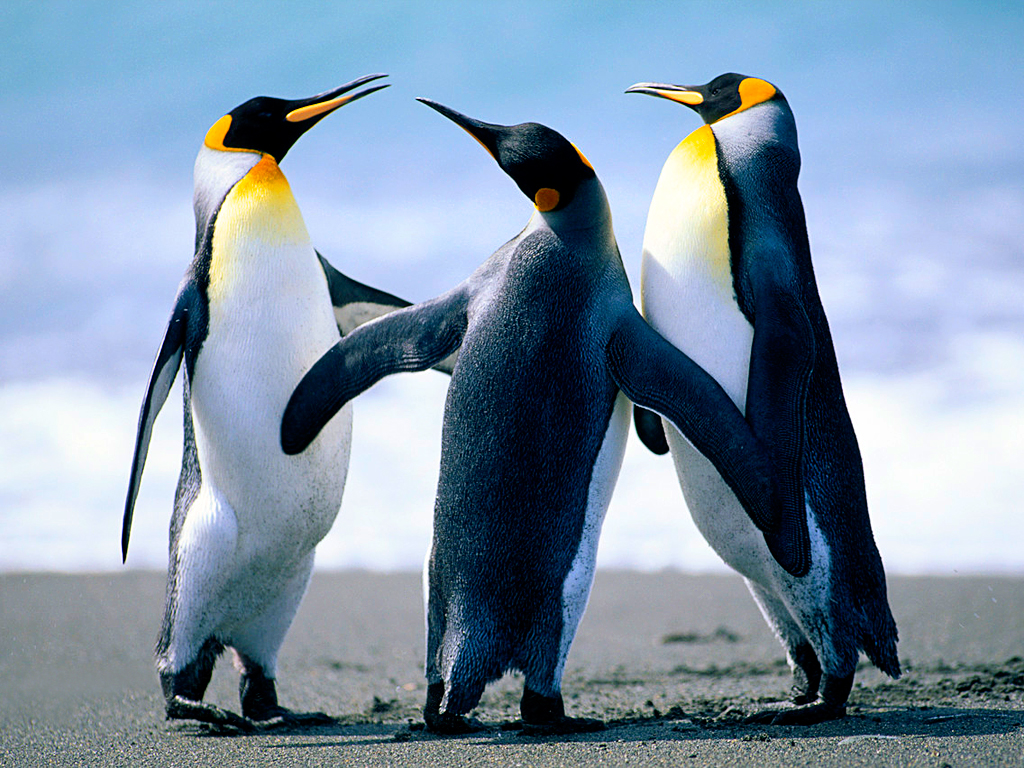
\includegraphics[scale=.50]{figures/Penguins.jpg}
\caption{TAMU figure - This is an example of a long figure title with a landscape figure.  Figure titles need to be single-spaced within and double spaced between in the list of figures.}
\label{fig:tamu-fig1-1}
\end{sidewaysfigure}
%%%%%%%%%%%%%%%%%%%%%%%%%%%%%%%%%%%%%%%%%%%%%%%%%%%%%%

More text here goes here.


Lorem ipsum dolor sit amet, consectetur adipiscing elit. Morbi augue urna, varius quis facilisis ac, imperdiet et nunc. Vestibulum ante ipsum primis in faucibus. 

\section{Current Processing Methodlogy}
Maecenas accumsan lobortis dui fringilla suscipit. Quisque congue fringilla dui, sed eleifend sapien fringilla euismod. Pellentesque habitant morbi tristique senectus et netus et malesuada fames ac turpis egestas. Maecenas venenatis posuere magna quis tempus. Cras at leo massa, eu ultricies tellus. Nunc nec dictum augue. Cum sociis natoque penatibus et magnis dis parturient montes, nascetur ridiculus mus. Phasellus purus felis, mollis id scelerisque in, viverra in elit. Nulla iaculis ultrices justo, ac pharetra nisl rhoncus pulvinar. Duis vitae mauris velit, in congue massa.

Donec lectus orci, bibendum ut blandit dignissim, molestie non eros. Praesent aliquet feugiat dignissim. Morbi porttitor sollicitudin nisl, non mollis quam ultrices sit amet. Cras feugiat lacinia diam ut convallis. Nam nec varius ante. Nunc a ultrices felis. Quisque luctus sapien et ligula ornare quis consequat urna aliquet. Vestibulum vulputate lorem a tellus auctor id commodo risus sodales. Suspendisse quis tortor a felis molestie laoreet ut a nunc. Donec gravida sapien eget mauris condimentum lacinia. Proin eu purus libero. Nullam augue mi, vestibulum in convallis eu, adipiscing ac arcu. Donec nisi libero, egestas et molestie in, mollis quis ipsum. Sed gravida quam sit amet ante tempus rutrum non in mi. Cras viverra facilisis eros, id vestibulum sapien malesuada eget. Maecenas imperdiet luctus nisi vitae suscipit.



Aliquam erat volutpat. Integer ut mauris elit. Nam et lectus vel neque vehicula commodo. Integer at risus ligula. Fusce mollis mauris sed lorem aliquam bibendum porttitor tellus blandit. Curabitur enim nibh, accumsan eu elementum id, rutrum a ipsum. Vivamus ultricies, elit id ornare iaculis, metus justo posuere quam, sit amet bibendum arcu dolor a eros. Sed in nisl nibh. Aenean egestas est ut tortor volutpat vehicula. Maecenas aliquet placerat nunc hendrerit dictum. In et nisi massa. Pellentesque luctus, sapien quis dignissim vulputate, sapien libero bibendum velit, vitae auctor ipsum nulla at augue. Nulla ac eros vitae tortor elementum vehicula.

Morbi tristique egestas placerat. Cras faucibus eleifend porta. Class aptent taciti sociosqu ad litora torquent per conubia nostra, per inceptos himenaeos. Ut a pellentesque neque. Donec sollicitudin metus varius nulla egestas laoreet. Duis non mauris ut nunc adipiscing volutpat. Nam vitae est sed turpis tristique varius. 

\subsection{This is a Very Long Subsection Title This is a Very Long Subsection Title}

More text
\subsection{Subsection}

Subsection text

\section{The Big Challege}

Section text
